% !TEX spellcheck = en
%% document class file for the preparation of a paper
%% for the International Conference ICCAS 2007
%% global option 'fleqn' ensures equations flush left.
%% set '10pt' and 'twocolumn' options.

\documentclass[fleqn,10pt,twocolumn]{ICCAS2012}
\usepackage{amsmath}

%%%%%%% set heading and page number heare %%%%%%%%%%
%\setcounter{page}{101}
\begin{document}

\title{A $n$-dimensional Convex Hull Approach for Fault Detection and Mitigation for High Degree of Freedom Robots Humanoid Robots}

\author{Kevin Lynch${}^{1}$, Daniel M. Lofaro${}^{2}$ and Paul Oh${}^{3}$}

\affils{  	${}^{1}$Department of Computer Science, \\
		${}^{2}$Department of Electrical and Computer Engineering, \\
		${}^{3}$Department of Mechanical Engineering,\\
Drexel University, Philadelphia, PA, USA\\
kml43@cs.drexel.edu, dml46@drexel.edu, paul@coe.drexel.edu\\
        }
\thanks{*This project was supported by the Drexel Autonomous Systems Lab (DASL) and by a National Science Foundation - Partnerships for International Research and Education grant (\#0730206). \\ 
*Hubo was designed and created by our partner Dr. Jun-Ho Oh, Department of Mechanical Engineering, Korean Advanced Institute of Science and Technology, Daejeon, South Korea.}% <-this %

%\thanks{ \noindent
%   This paper is supported by my funding agencies.
%  }
\abstract{
This work shows a plan for error state determination using N dimentional convexhull state maping.  This mapping determins if the robot is opperating in a normal state or is approaching an error state.  If the robot is in an error state a midigation dependent on the error state is chosen to move the robot back to the normal operating state.
}

\keywords{
    Humanoid Robotics, Fault Detection, Error Mitigation, $n$-dimensional Convex Hull
}

\maketitle

%-----------------------------------------------------------------------
\section{Introduction}

\textit{April 27th, 2010 - Philadelphia Convention Center (Main Hall):}  The robot handlers Daniel M. Lofaro 
and Robert Ellenberg were preparing the adult-size humanoid robot Jaemi Hubo\footnote{Jaemi Hubo Home Page: http://dasl.mem.drexel.edu/HUBO} at an outreach demonstration for the 
\textit{Arts \& Science Council} of Philadelphia.  During the dress rehearsal one of Jaemi's actuators failed 
during a demonstration of active balancing and she fell off of a 4 foot high stage.  The results of the impact 
can be found in Fig.~\ref{fig:fall} and on YouTube\footnote{Jaemi Hubo Fall: http://www.youtube.com/watch?v=DF8zAM4FLB4\label{link:fall}}.  
This annual event was a high profile fund raiser for the arts and science programs throughout the greater Philadelphia area and was covered widely by the media.  If this failure would have occurred during the actual event the 
aftermath would have been even more devastating.  In order for outreach events like this to successfully continue, methods 
for detecting failure states and quickly choosing appropriate mitigations must be developed.

All electro-mechanical systems have an inherent mean-time to failure.  Even with good maintenance these systems can fail without warning.  This work proposes ways to \textit{detect} when entering a failure state and ways of \textit{mitigating} such failures.  The adult-size humanoid robots Hubo2+ and Jaemi Hubo (KHR-4) are the primary test platforms for this proposed work.  All methods used are written in a broad scope so it can be applicable to other electro-mechanical systems.

\begin{figure}[t]
  \centering
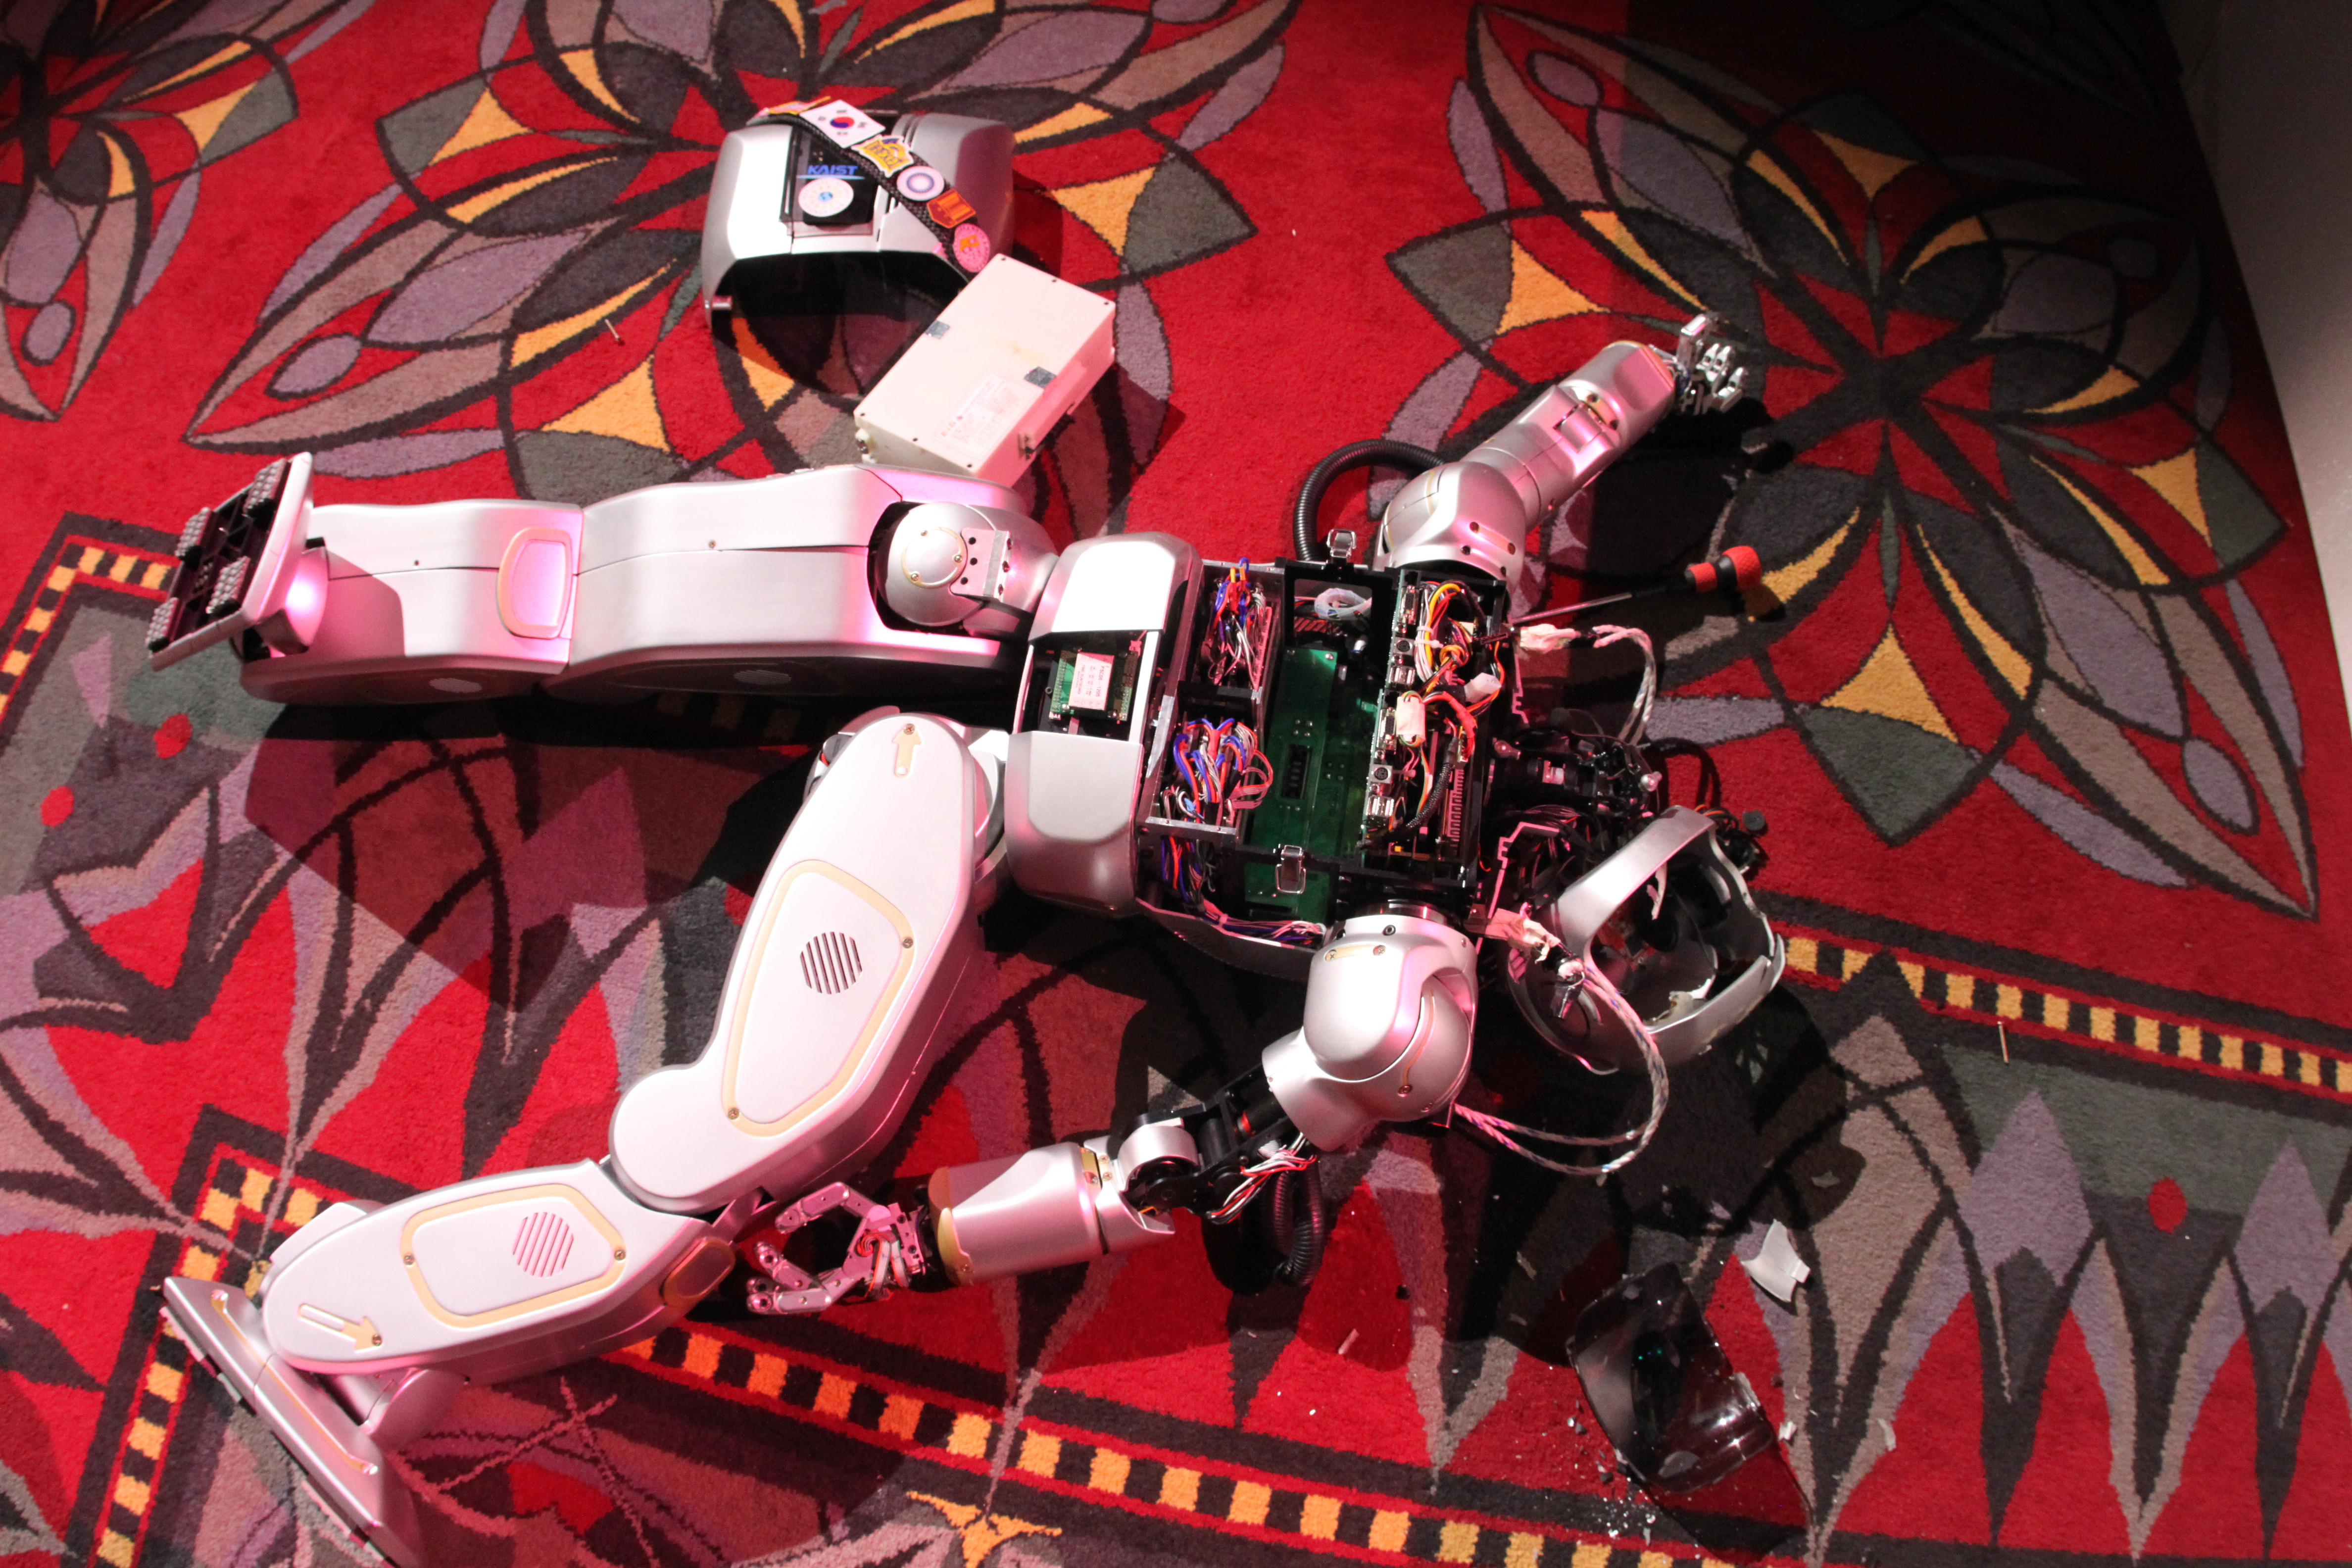
\includegraphics[width=1.0\columnwidth]{./pix/jaemiFall.png}
  \caption{-  Aftermath of the 4 foot fall Jaemi Hubo took after one of her actuators failed during operation.  A video with more images of the aftermath of the failure and further explanation of the event can be seen on YouTube.}%$^\ref{link:fall}$}
  \label{fig:fall}
\end{figure}  

Faults are difficult to detect before an executing system reaches a point of failure, as the first symptom of a fault is often system failure itself. While it is unrealistic to expect complex systems to be fault-free, actions such as resetting the system, quarantining specific components, or minimizing damage from the fault can be taken. Autonomic systems, an extension of fault tolerant systems, attempt to detect, diagnose, and mitigate faults quickly. These systems are inspired by the autonomic nervous system in the human body that monitors and regulates vital  functions of the body such as heart rate, respiration rate, and digestion. Similarly, an autonomic computer system is able to monitor itself and its environment and automatically adapt to complex changes. The goal of autonomic computing is to specify the desired state of a system using high-level objectives without detailing how to arrive at the state \cite{1160055,4061119,1301340}. By making intelligent decisions, autonomic systems free system administrators from low-level management and the intricacies of complex systems. Autonomic systems aim to be self-configuring, self-optimizing, self-healing, and self-protecting. These properties, collectively referred to as the self-* properties, are different views of the same self-man\-age\-ment property. For instance, a self-protecting system is ideally healing itself from faults while optimizing and reconfiguring itself to prevent other faults from reoccurring.

Outlined in this document is the proposed process to analyze the effects of faults on the complex system Jaemi Hubo/Hubo2+ (Fig.~\ref{fig:huboSch}).  We propose a method of injecting faults in a controlled environment so that we may easily analyze the effects of the faults on the normal operating state, Section~\ref{sub:Failure_State_Determination}.  Different mitigation techniques and their effect on the operating state will be explored and analyzed, Section~\ref{sub:mitigation_analysis}.

\begin{figure}[thpb]
  \centering
\includegraphics[width=1.0\columnwidth]{./pix/huboSch.png}
  \caption{Jaemi Hubo: 130cm tall 45kg (with battery and protective shell) 40 degree of freedom, high gain position controlled adult-size humanoid robot }
  \label{fig:huboSch}
\end{figure}



%We can never say that no parts will fail however we can know when they do and not have the entire system fail because of one part (reword).
%On April 27th, 2010: Jaemi Hubo was schedule to be apart of the \textit{Arts and Science Council} annual awards ceremony at the Philadelphia Convention Center.  During the dress rehearsal one of Jaemi's actuators failed ans she fell off of a 1.2 meter stage.








\section{Background}
\label{sec:background}
The techniques proposed in this work borrows from the bleeding edge work in
autonomic software engineering and computing.  The heart of autonomic computing
is anomaly detection, diagnosis, and mitigation. Autonomic systems perform 4
general tasks in a continuous closed loop: monitor components with the help of
sensors, interpret the monitored data, create a repair plan for system
adaptation, and execute this plan through effectors on the monitored system and
its environment. This is the MAPE (Monitor, Analyze, Plan, Execute) loop
\cite{1160055}. Fig.~\ref{fig:mape} illustrates how an autonomic element uses
this loop to manage a component.

\begin{figure}[tb]
  \centering
  \includegraphics[width=\columnwidth]{images/mape}
  \caption{- An autonomic element uses the MAPE control loop to monitor a
		component, analyze the its status with respect to a policy, plan how to
		meet the policy requirements, and execute a set of actions to do so.}
	\label{fig:mape}
\end{figure}

Autonomic approaches can be applied to many different types of systems,
particularly when focusing on fault detection and mitigation. self-healing
opearting systems \cite{DBLP:journals/ibmsj/AppavooHSWSKAEGGMORSX03,4351383}
protect against bit-flips and other transient hardware faults, and are able to
hot-swap components or firmware during runtime. At the application level, it is
possible to monitor the architecture requirements of a system and detect when
an architectural property (e.g. required connection bandwidth) falls outside of
an acceptable threshold \cite{Garlan2004}. If an invariant is violated, it
executes a strategy specifically designed to correct the violated
invariant. The strategies can reinitialize components and reconfigure the
system to recover from the violation and attempt to prevent the violation from
reoccurring. However, the applied strategies are \emph{ad hoc} solutions,
requiring developers and maintainers to understand and preempt the shortcomings
of the system, in much the same way they would manually debug and repair the
system.

\subsection{Fault Detection and Diagnosis}
\label{sub:fault_detection}
Previous approaches to the detection of software faults fall into two
categories, signature-based and
anomaly-based~\cite{al-nashif2008}. Signature-based methods detect faults by
matching measurements to known fault signatures. These techniques are used in
static fault-checking software such as the commercial antivirus software
McAfee~\cite{Mcafee} and Symantec~\cite{symantec}, as well as network intrusion
detection systems such as Snort~\cite{Roesch1999} and
Netstat~\cite{Vigna1999}. These techniques can also be used to detect recurring
runtime faults~\cite{Brodie2005}.

Typically, anomaly-detection techniques begin by collecting sensor measurements
of a normally behaving system. Then, they construct a representation of the
monitored system and compare any future measurements against that
representation. A common approach is to use metric correlations to quantify a
monitored system. During detection, if the correlations between metrics becomes
significantly different from the learned correlations, the system is classified
to be in a faulty state~\cite{zhen2006,zhao2009,Cohen2004,Jiang2009}.

Once a fault is detected, it must be correctly diagnosed. Bayesian Network
classifiers have been applied in several previous approaches to diagnosis
using. Ghanbari et al. propose an approach to anomaly diagnosis based on
Bayesian networks that are wholly or partially specified by a human user
\cite{Ghanbari2008}. Tree augmented naive bayesian classifiers are the basis
for software failure diagnosis in work by Cohen et al.~\cite{Cohen2004}. Zhang
et al. use ensembles of tree augmented naive Bayesian classifiers to diagnose
faults.~\cite{Zhang2005}. Other classification techniques have been used to
diagnose software faults. Chen et al.  offer an approach to the diagnosis of
failures in large-scale Internet service systems using decision trees
\cite{Chen2004}.  Duan et al.~\cite{Duan} propose an approach to diagnosis of
software failures that uses active learning to minimize the number of data
points that a human administrator must label.

In previous work it has been demonstrated that computational geometry can be
used to effectively detect system faults at
runtime\cite{stehle2010,shevertalov2010using}. The approach, introduced in the
work as Aniketos, is split into a training phase, and a monitoring
phase. During the training phase, the monitored system executes its normal
behavior and runtime data is periodically collected from sensors monitoring the
application, the operating system, and the hardware. Using these measurements,
we can construct an $n$-dimensional convex hull whose enclosing space
represents the normal execution of the monitored application, where $n$ is the
number of distinct metrics used. Figure~\ref{fig:class_hulls} shows an example
of a 2-dimensional convex hull.

\begin{figure}%[tb]
  \centering
  \includegraphics[width=\columnwidth]{images/class_hulls}
  \caption{- Building convex hulls for the diagnosis of faults (a) sample
		points from normal operation and two fault classes (b) Points inside of the
		convex hulls are diagnosed as normal or one of the fault classes. Points
		outside of all hulls are diagnosed as unknown faults.}
  \label{fig:class_hulls}
\end{figure}

During the monitoring phase, if a measurement point falls outside of this
enclosure, a fault is likely to have occurred. To properly mitigate the fault,
the problem must be diagnosed \cite{6100108} and a viable mitigation
selected. If measurement data is available for a set of known faults, then it
is possible to construct hulls for individual faults, or classes of
faults. During the monitoring phase, if a measurement falls within one of these
fault hulls we can determine which fault is likely occurring and apply a
mitigation.This approach is also capable of recognizing that an occurring fault
is not a type of fault that it has been trained to recognize. Typical
classification techniques, such as naive Bayes and voting feature
intervals\cite{Demiroz1997}, require that every sample be assigned a class from
a finite list of possible classes, which can cause drastic consequences if an
incorrect mitigation is selected. Our approach allows Aniketos to recognize
that a fault has occurred, but does not force Aniketos to label the fault as
one of the faults that it has been trained to recognize. One of the most
important features of a fault detection and diagnosis system is the ability to
handle new faults.

\begin{figure}[thpb]
  \centering
\includegraphics[width=1.0\columnwidth]{./pix/huboSch.png}
  \caption{Jaemi Hubo: 130cm tall 45kg (with battery and protective shell) 40
		degree of freedom, high gain position controlled adult-size humanoid robot
	}
  \label{fig:huboSch}
\end{figure}

\subsection{Fault Mitigation}
\label{sub:fault_mitigation}
Once a fault is detected and diagnosed a mitigation can be applied in an
attempt to bring the system back to a normal operating state. To select the
most appropriate mitigation to execute, mitigations must be evaluated based on
their performance cost, impact on the system, reliability, and how they affect
other mitigations locally as well as in the global environment. Given a set of
faults and a set of mitigations, it is possible to intuitively and empiracally
determine the best possible mitigation for a given fault. However, it is
impossible to plan for all possible fault scenarios, limiting the effectiveness
of mitigation selection.

Generally, when a fault is encountered there are several approaches that can be
taken. Reinitialization brings the whole system or part of the system, to its
initial state when a fault is detected.If a fault can be localized, it is
possible to progressively microreboot larger portions of the system until the
problem is resolved, starting with the most localized component
\cite{1251257}. A generalization of reinitialization, known as rollback,
restores the system to a previous checkpoint, undoing any environment changes
that may have been made \cite{1095833}. While this approach may not always be
feasible, in some cases, simply undoing the failing operation may be
sufficient. Often times, the system needs to be reconfigured to adapt to
changes in the system's environment. This can be done by tuning component
parameters, scaling components, replacing components, or removing components
entirely. Finally, in certain cases, it may be best to just accept the fault
and continue without mitigation.

It is important to understand that each of these approaches could have
potentially disastrous consequences on a given system. Different systems have
different objectives and costs risks associated with it. Similarly, each
mitigation has execution costs and risks associated with it. It is possible for
a selected mitigation to cause more faults, or increased downtime. If an
incorrect mitigation is applied, a cascading effect could quickly emerge.


\subsection{Humanoid Robot Fault Mitigation}
\label{sub:humanoidRobotFaultMitigation}
A typical fault for articulated robots is actuator failure.  Upon failure there
is no more power applied to the joint and the entire limb becomes under-actuated.
This is particularly hazardous to robots that require feedback to balance such as 
biped humanoid robots.  For biped humanoids these errors typically caused actuator 
over torque or hardware error resulting in loss of zero-moment-point
(ZMP) \cite{zmp35} causing a robot fall or collapse.  This is exceptionally
harmful to adult size humanoid robots due to their weight.  A common 
mitigation method described by Shin, J. et al.\cite{772398} from the Korean
Advanced Institute of Science and Technology (KAIST) changes the model of the
affected manipulator to one that is under-actuated.  This new model allows
the robust controller to continue to operate collision free (safe).

Current methods of mitigation of ZMP loss for biped humanoids been investigated
by Kiyoshi Fujiwara et al. \cite{4115653}.  These methods involve finding an
optimal falling trajectory that reduces the instantaneous force of the robot at
impact by creating multiple impact stages\cite{4399327}.  This method was fully
tested on an HRP-2FX (HRP-2P surrogate) and partially on an HRP-2P.  This work
did not include a method of determining a falling state, it is assumed that a
fall is in progress.  Additional work on detecting a fall and reducing fall
damage has been shown by Kunihiro Ogata et al.\cite{4755950}.  An active
shock-reducing motion reduces the impact damage by following the center of
gravity (COG) and attempting to keep it close to the ZMP support polygon.  The
falling state is determined when the predicted ZMP departs from the support
polygon. This method was tested on a miniature humanoid robot.  Additional work
on determining a fall state using machine learning techniques\cite{4813885}.
Reimund Renner et al. used parameter estimation of multiple sensors to detect a
falling state\cite{4058847}.


\section{Methodology}

Our proposed process is divided up into two distinct parts, failure state 
determination - Section~\ref{sub:FailureStateDetermination}~~ and mitigation - Section~\ref{sub:mitigationanalysis}~~.  The determination techniques designed to be 
wide in scope.  The midigation techniques are tailured towards adult-size
humanoid robots, specifically the Hubo platforms described in Section~\ref{sec:platform}.

 
\subsection{Platform}\label{sec:platform}
The robots that will be used in these experiments are the adult-size 
humanoid robots Jaemi Hubo and Hubo2+, see Fig.~\ref{fig:huboSch}.  
Each Hubo contains 40 degrees of freedom (DOF) and stands at a height of 130cm.
Each actuator has a high gain internal PID position control loop.  Reference positions are
commanded at 100hz over a half-duplex 1.0Mbps controlled area network (CAN).
Each actuator can feed back actual position, current through the actuator, and the actuator status 
(enabled or disabled).  Other metrics that are fed back are described in 
Table~\ref{table:states}.  

Currently we have direct access to seven Hubo's in total, six Hubo2+ and one Hubo2 (Jaemi Hubo).
Two of these robots will be used in these experiments for initial testing.




\subsection{Failure State Determination}\label{sub:FailureStateDetermination}




\subsection{Mitigation Analysis}\label{sub:mitigationanalysis}
The effectiveness of different mitigations has been analyzed on faults injected into two different systems typically used as benchmark applications in the software engineering community, RUBiS\footnote{http://rubis.ow2.org/} and Hadoop\footnote{http://hadoop.apache.org/}. RUBiS is a web application auction site running on the Apache Tomcat\footnote{http://tomcat.apache.org/} web server and serves page requests to hundreds of concurrently simulated clients. Hadoop is a distributed task manager that processes gigabytes of data across multiple nodes. We injected faults into both systems, the virtual machines they are running on, as well as the hosts managing the virtual machines. The faults consumed either processor, memory, disk, database, or network resources in the respective components. We applied generic mitigations that restarted various components, migrated the components to new hosts or virtual machines, or did nothing. The effectiveness of each fault-mitigation pair was analyzed on each system to generate a mapping of faults to mitigations. Using this knowledge, if a fault is later encountered, the best mitigation can be applied with a high chance of success. If a particular mitigation cannot be applied in that instance, then the next best mitigation may be selected, and so forth.

% When an anomaly occurs, multiple mitigations may be triggered at once. For instance, if a hardware failure is detected on a host, all process should be migrated to another machine and diagnostic utilities should be run on the machine.

A naive observer would expect the two systems to have nearly identical fault-mitigation mappings. However, in our testing on software based systems the generated mappings varied greatly in the effectiveness of the mitigations on a particular fault.  RUBiS is a typical web application that receives requests from clients and processes results returned from a database. Little processing is being done by RUBiS or its host machine, so even though a processor intensive fault may be using up many cycles in the process or the host, there is no noticeable effect on the request processing rate. As a result, any mitigation applied would result in more down time than if no mitigation were to be applied. Unlike RUBiS, Hadoop is much more processor intensive. Any host level fault that is slowing down the system will adversely affect the completion time for the task. Another major difference is that RUBiS, like many other request driven systems, can easily be restarted to temporarily address fault symptoms, while restarting Hadoop typically means losing already processed results.  We expect similar results when applying this method to the complex electro-mechanical platforms Jaemi Hubo/Hubo2+.

The generated fault-mitigation mappings for the two systems offer insight into their respective natures. On the surface, both software systems operate like typical servers, waiting for requests or tasks, and processing them in a timely fashion. However, the way the requests are handled results in faults manifesting in different ways. Even though a fault may be detected, the obvious mitigation is not always the best. This approach to mitigation analysis, will offer valuable insight into the true effectiveness of mitigations when faults occur in Hubo.




\subsection{none}












\section{Expected Results}
\label{sec:expResults}

It is expected that the recorded metrics will converge and give us a well defined convex hull for normal operating state.  Failure states such as ZMP loss or  actuator over current is also expected to create a well defined hull due to it's tight correlation with the kinematics and sensor data.  Failures that are not tightly correlated other metrics, such as actuator zero or actuator status, are not expected to form a well defined hull.  Similar to the software system it is expected that the mitigation methods will very from platform to platform despite having the same faults present.

\section{Conclusion}
Through the failure at the Philadelphia Convention Center it has been shown that there is a need for fault state detection and mitigation.
It has been shown that Aniketos system is capable of creating an $n$-dimensional convex hull describing proper running states and failure states on software system.  A plan has been described to apply Aniketos to a physical platform which included injecting faults into the physical system and creating the convex hull from the recorded sensor and state data.  The expected results are described in Section~\ref{sec:expResults} and are based on the results from the software testing.

%\subsection{Faults}
\label{sec:faults}
The states that we will be analyzing for the creation of the convex hull for
the fault detection mapping fall into four categories, faults, status, low
level feedback, high level feedback.  A list of the


%\input{mitigation.tex}


%%%%%%%%%%%%%%%%% BIBLIOGRAPHY IN THE LaTeX file !!!!! %%%%%%%%%%%%%%%%%%%%%%
%%---------------------------------------------------------------------------%%
%
%\begin{thebibliography}{99}


%\bibliographystyle{plain}
%\bibliography{mit}

\bibliographystyle{IEEEtran}
%\bibliographystyle{plain}
\bibliography{mit}{}


%\end{thebibliography}

%
%%--------------------------------------------------------------------%%

\end{document}
